\documentclass[11pt,letterpaper]{article}
\usepackage[margin=.83in,top=.81in,bottom=.78in,headheight=14pt,headsep=16pt]{geometry}
\usepackage{amsmath,amssymb,booktabs,array,xcolor,tikz,fancyhdr,hyperref}
\usetikzlibrary{arrows.meta,positioning}
\definecolor{ink}{HTML}{1C3449}\definecolor{green}{HTML}{136351}\definecolor{muted}{HTML}{49616F}
\definecolor{pale}{HTML}{E9F2ED}\definecolor{red}{HTML}{AA4538}\definecolor{blue}{HTML}{255E97}
\hypersetup{colorlinks=true,linkcolor=green,urlcolor=blue,pdftitle={Four clues and Fibonacci counts},pdfauthor={Research note prepared for Dominic Dabish}}
\pagestyle{fancy}\fancyhf{}\fancyhead[L]{\sffamily\footnotesize\color{green} GRAPH COLORING}
\fancyhead[R]{\sffamily\footnotesize\color{muted} EXTENSION AND MODULAR COUNTING}
\fancyfoot[L]{\sffamily\footnotesize\color{muted} Research note for Dominic Dabish \quad / \quad 21 November 2026}
\fancyfoot[R]{\sffamily\footnotesize\color{muted}\thepage}
\setlength{\parindent}{0pt}\setlength{\parskip}{5pt}\setlength{\emergencystretch}{1em}
\setlength{\abovedisplayskip}{7pt}\setlength{\belowdisplayskip}{7pt}
\newcommand{\secx}[1]{\section[#1]{\color{ink}#1}}
\newcommand{\subx}[1]{\par\medskip{\large\bfseries\color{green}#1}\par\nobreak}
\newcommand{\run}[1]{\par\smallskip{\bfseries\color{ink}#1}\quad}
\newcommand{\boxx}[1]{\par\smallskip\colorbox{pale}{\parbox{\dimexpr\linewidth-2\fboxsep\relax}{\vspace{3pt}#1\vspace{3pt}}}\par\smallskip}
\newcommand{\sat}{\#\mathrm{SAT}}\newcommand{\Z}{\mathbb Z}\newcommand{\FF}{\mathbb F}
\newcommand{\refx}[2]{\href{#1}{#2}}
\begin{document}
\pdfbookmark[1]{Main results}{main}
{\sffamily\small\color{muted} COMPUTATIONAL COMPLEXITY \hfill WORKING MANUSCRIPT}\par
{\fontsize{24.88}{29}\selectfont\bfseries\color{ink}Four clues and Fibonacci counts\par}
{\large\color{muted} A Boolean formula encoded in the number of edge colorings\par}
\medskip
A proper edge coloring of a cubic graph uses red, blue and green once at every vertex. All graphs used as outputs below are connected, simple, bipartite and cubic. Color names are distinguished. A clue fixes the color of one edge. Write \(Z\) for the number of full colorings respecting every clue.
\subx{A reduction with a supplied solution}
For every CNF formula \(F\) on \(n\) variables, the construction produces a graph, two red and two blue clues with disjoint endpoints, a valid full coloring, an odd Fibonacci number \(m>2^n\), and a unit \(u\) modulo \(m\). The four clues form the full boundary between two connected pieces. The construction takes polynomial time and
\[
                   \boxed{\qquad \sat(F)=(u^{-1}Z)\bmod m. \qquad}
\]
The residue is taken between zero and \(m-1\). Thus divisibility by \(m\) decides whether \(F\) is unsatisfiable. Every output already comes with a witness that \(Z>0\).
\begin{center}
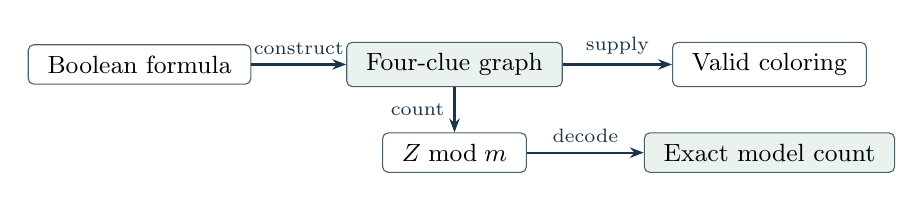
\begin{tikzpicture}[x=1cm,y=1cm,every node/.style={font=\small},
 item/.style={draw=muted,rounded corners=2pt,inner xsep=7pt,inner ysep=4pt},
 arr/.style={-{Stealth[length=5pt]},thick,ink}]
\node[item] (f) at (0,0) {Boolean formula};
\node[item,fill=pale] (g) at (4.0,0) {Four-clue graph};
\node[item] (w) at (8.0,0) {Valid coloring};
\node[item] (z) at (4.0,-1.12) {$Z\bmod m$};
\node[item,fill=pale] (c) at (8.0,-1.12) {Exact model count};
\draw[arr] (f)--node[above,font=\scriptsize]{construct} (g);
\draw[arr] (g)--node[above,font=\scriptsize]{supply} (w);
\draw[arr] (g)--node[left,font=\scriptsize]{count} (z);
\draw[arr] (z)--node[above,font=\scriptsize]{decode} (c);
\end{tikzpicture}\end{center}
\subx{Three consequences}
\begin{tabular}{@{}p{.28\linewidth}p{.655\linewidth}@{}}
\toprule
Question & Result obtained here \\ \midrule
Four clues on a bond & Exactly four of the six ways to choose the two red edges extend. All four attainable counts have the same parity. \\[4pt]
Fixed prime, no clues & The labeled count is zero modulo 2 and 3. Computing it modulo any fixed prime \(p\ge5\) is \(\#_p\mathrm P\)-complete. \\[4pt]
Fixed odd modulus & A single red clue suffices for \(\#_m\mathrm P\)-complete counting for every fixed odd \(m\ge3\). This holds also with the four disjoint bond clues and a supplied coloring. \\
\bottomrule
\end{tabular}
\subx{Where this sits in the literature}
Hong's 2021 talk listed exact counting on cubic bipartite graphs as open [1]. Boehmer and coauthors proved exact hardness in 2023, including the planar case [2]. This note concerns residues, the explicit SAT decoder, and sparse prescribed colors. The source reduction uses Faben's independent-set framework [3]. Publication priority for these refinements and independent review of this manuscript remain outstanding. P versus NP remains open [6].
\newpage
\secx{Which four-clue cuts can be colored?}
Let \(G=(L,R;E)\). A \emph{bond} is a cut whose removal leaves exactly two connected shores. On a four-edge bond choose two edges red and the other two blue. Viewed from one shore, two of its four endpoints are in \(L\) and two in \(R\), counted with multiplicity. Indeed their signed difference equals three times the shore's bipartition imbalance. Among \(-4,-2,0,2,4\) only zero is divisible by three.
\boxx{A placement extends if and only if the two red ends meet opposite bipartition classes on a shore. The two blue ends then do likewise on both shores. Four of the six placements pass.}
\run{Necessity.} In any one color each internal edge accounts for one vertex from each side. Hence the difference of counts of boundary ends of that color must equal the shore's imbalance, which is zero here.
\run{Sufficiency.} Close the red pair on a shore with a new edge \(e\) and the blue pair with \(f\). The resulting bipartite cubic multigraph is regular. The shore contains a simple path between the endpoints of \(e\). This path plus \(e\) is an even cycle avoiding \(f\), including the possible case of a two-edge cycle. Start each edge with multiplicity one. Alternately add and subtract one along this cycle, adding on \(e\). Every vertex still has degree three counting multiplicity. The resulting bipartite multigraph decomposes into three perfect matchings. Two of them use \(e\), and only one uses \(f\). Take a matching using \(e\) and avoiding \(f\) as red in the original closed shore. Its complement is a union of even cycles. Orient the alternating blue and green colors to give \(f\) blue. Glue the two shore colorings.
\run{A general four-edge cut.} A connected regular bipartite cubic graph has no bridge, by perfect-matching decomposition or bipartition balance on a one-edge cut. Thus each component of either shore uses at least two of its four ends. The possible splits are four, or two plus two. In a two-end component the ends lie in opposite bipartition classes and must have the same color. Capping them by one edge and permuting a full coloring suffices. The componentwise balance condition for each color is therefore exact on every four-edge cut. Testing cut membership, components and balances takes \(O(|V|+|E|)\) time. Constructing a coloring uses bipartite matching.
\subx{A parity identity}
In a connected four-end shore with two ends of each side, choose an internal perfect matching. Such a matching exists as the third color in a mixed extension just proved. At a matched pair, sum over the color on its joining edge. Modulo 2 its local constraint equals the sum of the two input-to-output pairings. Distinct matching pairs of colors admit exactly one pairing. Four equal colors admit two pairings, which sum to zero, agreeing with the original constraint. Every other boundary pattern contributes zero. Each choice of pairings over the matching joins the two input ends bijectively to the two output ends and forms some internal loops. Each loop contributes \(3\equiv1\pmod2\). For fixed unequal input colors exactly one of the two possible output orders fits each choice. Their counts sum to \(2^{|M|}\equiv0\pmod2\). Thus both mixed orders have equal parity. Multiplying the contributions of the two shores proves the bond parity claim.
\newpage
\secx{A 16-vertex obstruction to fractional coloring}
The usual linear feasibility test has variables \(x_{e,c}\ge0\), edge equations \(\sum_c x_{e,c}=1\), vertex equations \(\sum_{e\ni v}x_{e,c}=1\) for each color, and \(x_{e,c}=1\) on each clue. With at most three clues drawn from two colors, fractional feasibility guarantees extension. Choose the majority color as red. Its fractional matching lies in the bipartite perfect-matching polytope with forced and forbidden edges, hence an integral red matching exists there. At most one blue edge remains to orient in its complementary even cycles.
\subx{Four disjoint clues already defeat the test}
The left vertices are rows 1 through 8, the right vertices letters A through H. Each table entry is a neighbor followed by \(2(x_R,x_B,x_G)\). The clues in order are red \(1B\), blue \(2G\), red \(5H\), and blue \(8D\).
\begin{center}\renewcommand{\arraystretch}{1.11}
\begin{tabular}{c@{\quad}lll}\toprule
Row & First neighbor & Second neighbor & Third neighbor \\ \midrule
1 & B 200 & C 011 & E 011 \\
2 & D 200 & F 002 & G 020 \\
3 & B 011 & F 110 & G 101 \\
4 & A 101 & B 011 & C 110 \\
5 & A 020 & D 002 & H 200 \\
6 & A 101 & F 110 & H 011 \\
7 & E 110 & G 101 & H 011 \\
8 & C 101 & D 020 & E 101 \\ \bottomrule
\end{tabular}\end{center}
Every triple sums to two. At every row and every letter, its three triples sum to \((2,2,2)\). Dividing by two proves fractional feasibility using only integer checks.
\run{Why an integral coloring is impossible.} In a red perfect matching, rows 1 and 5 must choose B and H. Only row 2 can supply D, since \(8D\) is blue. The remaining five rows and five columns form one ten-cycle of red candidates. Its two alternating halves give every possible red matching. The letter strings below list the selected columns in row order.
\begin{center}\begin{tabular}{@{}lcc@{}}\toprule
Red matching & Complementary cycle length & Steps from one blue clue to the other\\ \midrule
\texttt{BDFCHAGE} & 16 & 7 \\
\texttt{BDGAHFEC} & 16 & 7 \\ \bottomrule
\end{tabular}\end{center}
In either complementary cycle the blue positions have opposite parity. The complete graph has 120 labeled colorings before the clues. Deleting one clue restores respectively 4, 2, 5 and 4 extensions in the order listed above. These four edges lie outside the cut case on page 2.
\run{Spacing.} To separate the clues arbitrarily far, replace each prescribed edge by a chain of an even number of copies of \(K_{3,3}\) minus one edge, pinning its middle connector. A two-edge cut transmits one color, and every common color extends. The two degree-two vertices in each copy are at distance three. Full-coloring feasibility is preserved. The fractional certificate lifts by choosing on each substituted chain an integral local coloring with the prescribed common color. The untouched weights stay feasible. This gives arbitrarily spaced four-clue failures.
\newpage
\secx{Four terminals and two Fibonacci numbers}
A box has two unconnected edge ends at left-part vertices, with ordered colors \((a,b)\), and two at right-part vertices, with colors \((c,d)\). Such open-edge boundary states are standard for cubic multipoles [5]. The boxes here have equally sized parts. Color balance forces \(\{a,b\}=\{c,d\}\) as multisets. By palette symmetry there are three possible counts: \(A\) for all equal, \(B\) for distinct colors in the same order, and \(C\) for distinct colors exchanged. Our boxes have \(B=C\).
\begin{center}
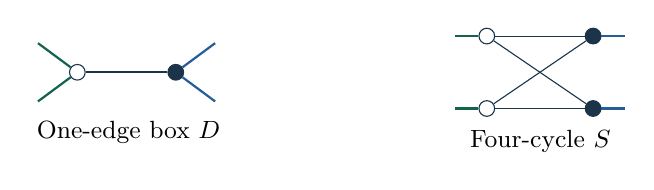
\begin{tikzpicture}[x=1cm,y=1cm,every node/.style={font=\small},dot/.style={circle,draw=ink,fill=white,inner sep=2pt}]
\begin{scope}[xshift=.1cm]
\node[dot] (l) at (0,0) {};\node[dot,fill=ink] (r) at (1.25,0) {};
\draw[thick,ink](l)--(r);\draw[green,thick](-.5,.37)--(l)--(-.5,-.37);\draw[blue,thick](1.75,.37)--(r)--(1.75,-.37);
\node at (.65,-.76) {One-edge box \(D\)};
\end{scope}
\begin{scope}[xshift=5.3cm]
\node[dot] (a) at (0,.46) {};\node[dot] (b) at (0,-.46) {};\node[dot,fill=ink] (c) at (1.35,.46) {};\node[dot,fill=ink] (d) at (1.35,-.46) {};
\foreach \v in {a,b} {\foreach \w in {c,d} {\draw[ink] (\v)--(\w);}}
\draw[green,thick](-.4,.46)--(a);\draw[green,thick](-.4,-.46)--(b);
\draw[blue,thick](c)--(1.75,.46);\draw[blue,thick](d)--(1.75,-.46);
\node at (.68,-.88) {Four-cycle \(S\)};
\end{scope}
\end{tikzpicture}
\end{center}
\(D\) consists of one edge whose endpoints carry two ends each. Its counts are \((0,1,1)\). The square \(S=K_{2,2}\) has one end per vertex and counts \((2,1,1)\). In the drawing an intersection of two drawn lines has no vertex.
\run{One iteration.} Begin with \(Q_0=D\). In \(Q_k\) retain its first left and right ends. Join its second left end to the first right end of a fresh \(D\), and its second right end to the first left end of that \(D\). The two other ends of \(D\) become the new second pair. Next join both right ends to the two left ends of a fresh square \(S\) in order. Its right ends are the final outputs.
\run{The recurrence.} Suppose \(Q_k\) has counts \((A,B,B)\). The first operation gives \((2B,A+B,B)\). In the all-equal case the pair joined to \(D\) must use a common different color, giving two choices. For aligned mixed external colors the two choices give weights \(A\) and \(B\). For crossed mixed colors the internal ordering is fixed, giving \(B\). Appending the square doubles the all-equal weight and adds the two mixed weights for either output order. Hence
\[
      A_{k+1}=4B_k,\qquad B_{k+1}=A_k+2B_k,\qquad
      A_k=2^{k+1}F_k,\quad B_k=2^kF_{k+1}.
\]
Here \(F_0=0,F_1=1\). The graph has \(2+6k\) vertices and stays simple and connected. For \(k\ge1\) the four terminal vertices are distinct.
\run{The filter.} Given odd \(m\ge3\), choose the least \(k\) with \(F_{k+1}=0\bmod m\). The map \((x,y)\mapsto(y,x+y)\) is invertible on \((\Z/m)^2\), so its orbit returns to \((0,1)\) within \(m^2\) steps. Consecutive Fibonacci numbers are coprime. Thus \(a=A_k\bmod m\) is a unit, while each mixed count is zero modulo \(m\). For \(m=5\), \(Q_4\) has 26 vertices and counts \((96,80,80)\). All three patterns really occur. Only the all-equal pattern contributes to the residue.
\newpage
\secx{Encoding independent sets in a closed graph}
Let \(J=(U,V;E_J)\) be any simple bipartite graph, with \(I(J)\) independent sets including the empty one. Form a connected graph \(P\) with a palette triangle \(r,b,g\). Add \(J\), connect every \(U\)-vertex to \(g\), and every \(V\)-vertex to \(b\). Fix the triangle's colors in that order. Each source vertex may be red (selected) or take its unique permitted alternative. A source edge forbids selecting both ends. This gives exactly \(I(J)\) vertex colorings with the palette fixed and \(6I(J)\) with it free.
\subx{Replace each incidence by a four-terminal box}
For each edge \(vw\) of \(P\) create one left and one right comparison vertex joined by an edge. Build a \(Q_k\) for each of its two endpoints. Join the box's first output to the left comparison vertex, its first input to the right comparison vertex. For each vertex of \(P\) arrange its incidence boxes in a cyclic order. Join the second output of each box to the second input of the next, including a return wire for a degree-one vertex. These simple bipartite graphs have \(2e+(2+6k)q\) vertices, where \(e=|E(P)|\) and \(q=2e\). Each vertex has degree three. Each comparison connects its two endpoint groups, so the graph is connected. A return wire spans distinct box vertices and duplicates no internal edge: the final right ends lie in the appended square and the second left end lies in the added one-edge box.
\run{Count with no clues.} Sum over the colors on the wires outside each box. The local counts multiply. Modulo \(m\) any mixed box contributes zero. With every box monochromatic on its four ends, each ring has one color. At a comparison the two ring colors must differ and determine the joining edge's color uniquely. Hence \(Z_0\equiv 6a^q I(J)\pmod m\).
\run{One clue.} Fix one connector on the \(r\)-ring to red. Two permutations of the remaining palette survive, giving \(Z_1\equiv 2a^q I(J)\pmod m\). Indeed \(Z_1=Z_0/3\) over the integers by global palette symmetry.
\run{Four disjoint clues in one bond.} Take the cube as two four-cycles joined by four corresponding edges. Pin those four connecting edges, in cyclic order, red, red, blue, blue. There is exactly one full coloring: around each square the internal colors are blue, green, red, green. Remove the internal red edge of one square. Substitute this two-end cube for the preceding red ring connector, leaving only the four cube clues pinned. Both new terminal edges must have the same color by the two-edge cut. Closing the punctured cube restores its unique coloring and forces that color to be red. Thus the four-clue count equals \(Z_1\) exactly, at a cost of eight vertices. The untouched square is one shore of the four-edge bond. The other shore remains connected, since the broken square is a path and the original connector can be replaced by that path. All four clues form a matching.
\begin{center}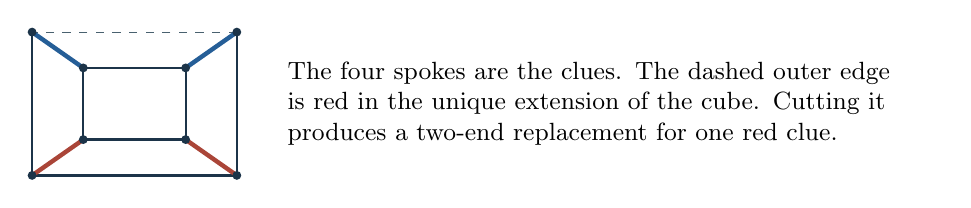
\begin{tikzpicture}[x=.65cm,y=.65cm,every node/.style={font=\small}]
\coordinate (b0) at (0,0);\coordinate (b1) at (4,0);\coordinate (b2) at (4,2.8);\coordinate (b3) at (0,2.8);
\coordinate (t0) at (1,.7);\coordinate (t1) at (3,.7);\coordinate (t2) at (3,2.1);\coordinate (t3) at (1,2.1);
\draw[ink,thick] (b3)--(b0)--(b1)--(b2);\draw[muted,dashed] (b2)--(b3);
\draw[ink,thick] (t0)--(t1)--(t2)--(t3)--cycle;
\draw[red,line width=1.6pt] (b0)--(t0) (b1)--(t1);
\draw[blue,line width=1.6pt] (b2)--(t2) (b3)--(t3);
\foreach \v in {b0,b1,b2,b3,t0,t1,t2,t3}{\fill[ink] (\v) circle (1.6pt);}
\node[anchor=west,align=left,text width=8.2cm] at (4.8,1.4) {The four spokes are the clues. The dashed outer edge is red in the unique extension of the cube. Cutting it produces a two-end replacement for one red clue.};
\end{tikzpicture}\end{center}
\boxx{A witness is available before any counting. Use the empty independent set, its fixed palette, and four equal boundary colors on every box. Since \(A_k>0\), each box extends. To construct the local coloring, cap the two pairs with forced edges of the common color, find a perfect matching containing both, and alternate the other two colors on its complement.}
\newpage
\secx{From CNF to a single diagnostic remainder}
Here is a self-contained modular source reduction following Faben's variable construction [3]. It works over every odd \(m\ge3\), including prime powers. It also specifies how large \(m\) needs to be to recover the ordinary model count.
\run{A path enforcing a disjunction modulo \(m\).} Use \(P_{k-1}\), the path on \(k-1\) vertices, with one endpoint adjacent to every candidate in a given set. That set lies in one bipartition class. If no candidate is selected in an independent set, the path contributes \(F_{k+1}\equiv0\). If at least one is selected the endpoint is excluded and the path contributes \(F_k\), a unit. The independent-set count of a path on \(j\) vertices is \(F_{j+2}\) by the recurrence at its endpoint.
\run{Variables and clauses.} For a variable put literal vertices \(t_i,f_i\) on the left and partners \(p_i,q_i\) on the right, with edges \(t_ip_i,f_iq_i\). Add one path constraint requiring a selection from \(\{t_i,f_i\}\) and another from \(\{p_i,q_i\}\). The only contributing choices on the four original vertices are \(\{t_i,q_i\}\) and \(\{f_i,p_i\}\). For each clause add a path requiring a choice from its literal vertices. Multiple occurrences use a single attachment per distinct literal. An empty clause gives zero residue. Unused variables retain both choices. With \(s\) clauses, \(d=2n+s\) such paths, and the four-clue construction of page 5, this proves
\[
                   Z\equiv u\,\sat(F)\pmod m,\qquad
                   u=2 a^q F_k^{d}\pmod m.
\]
Every factor of \(u\) is invertible modulo \(m\). For fixed \(m\) the graph has linear size in the formula's variable, clause and literal-occurrence counts. Counting extensions modulo \(m\) is in \(\#_m\mathrm P\) by guessing a labeled coloring. Counting accepting witnesses modulo \(m\) reduces to modular \(\#\)SAT by the usual parsimonious circuit encoding, so the displayed one-instance identity proves completeness. For no pins the leading factor is 6; it is invertible for primes above 3. At primes 2 and 3 the six free palette permutations force zero on every nonempty cubic graph.
\subx{Choose the modulus from the formula}
Take the first odd Fibonacci number \(F_t\ge3\) exceeding \(2^n\). Fibonacci numbers at least double every two indices after the first, and every third Fibonacci number is even. Thus \(t=O(n+1)\) and \(F_t\) has \(O(n+1)\) bits. The first positive Fibonacci multiple of \(F_t\) is \(F_t\) itself, so the selected filter depth is exactly \(t-1\). Both graph constructions are polynomial in the original input length (with variables explicitly represented). After inversion of \(u\) the least nonnegative residue equals the ordinary \(\sat(F)\). In particular, a uniform polynomial-time divisibility algorithm for these promised graph/modulus pairs would decide SAT in polynomial time.
\run{A matched pair.} The formulas \((x)\land(x)\) and \((x)\land(\neg x)\) each give a 1,142-vertex graph with a supplied coloring. For both, \(m=3\) and \(u=2\). The graph residues are respectively 2 and 0, decoding to exactly 1 and 0 satisfying assignments.
\newpage
\secx{Latin rectangles and independent checks}
For a Latin rectangle with \(N-3\) complete rows and \(N\) columns on \(N\) symbols, put an edge between a column and a symbol still missing there. This is a simple cubic bipartite graph. Coloring an edge by the row where that symbol will be used gives a bijection between completions and proper labeled 3-edge-colorings [4]. Conversely, from the cubic graph fill the first \(N-3\) rows by decomposing its regular bipartite complement into perfect matchings. One edge clue fixes one last-row cell's symbol.
\run{A threshold in rows remaining.} With two rows remaining, the residual graph is a union of even cycles. Test the two orientations independently on each cycle and multiply the numbers allowed. This handles any extra prescribed cells. With three rows remaining and no additional cells, modular counting is complete for every fixed prime \(p\ge5\). With one extra cell, or with four cells in the two prescribed rows of our family, modular counting is complete for every fixed odd modulus. A valid completion can be supplied. These reductions concern Latin row and column restrictions. Adding Sudoku boxes changes the problem.
\subx{Checks against the actual graphs}
\begin{tabular}{@{}p{.26\linewidth}p{.69\linewidth}@{}}\toprule
Check & Observed result \\ \midrule
Local counts & Direct integer contraction of all 81 terminal assignments at each of 25 depths. Arithmetic checks for all 150 odd moduli from 3 through 301. \\[3pt]
Closed graph residues & 320 independently contracted raw graphs, up to 1,526 vertices, for five moduli and four clue counts. All predicted residues and all supplied witnesses agreed. A separate block-ordered contraction matched the raw results. \\[3pt]
CNF decoder & 30 complete reductions at moduli 3, 5 and 9, up to 22,364 vertices. A block-ordered graph contraction recomputed the local tensors and decoded every truth-table count. Four further exact-decoder runs reached 80,846 vertices. Two equal-order SAT/UNSAT graphs were also counted directly over the integers. Both counts have 105 digits. \\[3pt]
Four-edge cuts & All 5,532 two-and-two placements on 922 cuts of 33 graphs agreed with full-coloring enumeration. All 921 bonds had the predicted common parity over their four feasible placements (538 odd, 383 even). \\[3pt]
Latin conversion & Direct enumeration for 69 small rectangles matched raw graph counts. Full supplied squares of orders 130, 166 and 274 passed all row, column and clue checks. \\ \bottomrule
\end{tabular}
\run{Worked count.} A source \(J\) consisting of one edge has three independent sets. At \(m=5\) the four-clue graph has 332 vertices and \(q=12\). Its integer count is \(563814076452372728421176836096\), congruent to \(1=2\cdot3\bmod5\). This value was recomputed directly from the 498 edges and their clues.
\run{Remaining questions.} The general extension decision with four arbitrarily placed clues remains unresolved by these arguments. The certificate on page 3 rules out the elementary linear relaxation. The parity identity on a bond compares placements; it leaves the difficulty of computing their common parity open here. The fixed-prime classification is for unembedded graphs and gives no general polynomial-time SAT algorithm.
\newpage
\pdfbookmark[1]{References and replication}{refs}
{\LARGE\bfseries\color{ink}References and replication\par}
\smallskip
\begin{enumerate}
\item Letong Hong. \refx{https://cdc2020-math.uniri.hr/wp-content/uploads/2021/07/talk_hong.pdf}{A Markov chain on the solution space of edge-colorings of bipartite graphs}. Combinatorial Designs and Codes, 2021. The section on previous results explicitly poses the cubic bipartite counting problem.
\item Niclas Boehmer, Jin-Yi Cai, Piotr Faliszewski and coauthors. \refx{https://ojs.aaai.org/index.php/AAAI/article/download/25684/25456}{Properties of position matrices and their elections}. AAAI 2023, 5507--5514. Theorem 2 proves exact counting hardness and the authors record its planar version.
\item John Faben. \refx{https://arxiv.org/abs/0809.1836}{The complexity of counting solutions to generalised satisfiability problems modulo \(k\)}. 2008, especially Theorem 3.7 and the two-pair variable construction. Page 6 gives the path realization and the full multiplier used in this note.
\item Letong Hong and István Miklós. \refx{https://real.mtak.hu/191308/1/2103.11990v1.pdf}{A Markov chain on the solution space of edge-colorings of bipartite graphs}. Author manuscript, 2021; journal version in \emph{Discrete Applied Mathematics} (2023). Section 4 gives the Latin rectangle correspondence.
\item M. A. Fiol and J. Vilaltella. \refx{https://doi.org/10.37236/3629}{Some results on the structure of multipoles in the study of snarks}. \emph{Electronic Journal of Combinatorics} 22 (2015), P1.45. Background on boundary states and the parity lemma.
\item Clay Mathematics Institute. \refx{https://www.claymath.org/millennium/p-vs-np/}{P vs NP}. Millennium Prize problem status, consulted 21 November 2026.
\end{enumerate}
\subx{Running the companion archive}
\texttt{sat\_to\_four.py} accepts DIMACS CNF. With \texttt{--exact} it outputs the graph and prints the decoder modulus and inverse. With \texttt{--witness} it also writes one valid coloring. Its Python dependencies are all in the standard library. \texttt{raw\_counter.py} reads the resulting explicit graph and contracts its all-different tensors. The raw exact counter can take exponential time. The companion includes a second contraction order, an independent exhaustive edge-colorer, the small linear-program certificate and a Latin converter. See \texttt{README.md} for executable commands and the five check logs.
\subx{Scope and attribution}
The exact counting theorem in [2], modular counting source in [3] and correspondence in [4] are prior work. This note supplies the four-cut proof, a half-integral obstruction with two red candidates, a Fibonacci transfer construction, and an explicit fixed- and growing-modulus reduction. The literature search did not establish publication priority. Finite checks support the implementations; the universal statements depend on the mathematical arguments above.
\end{document}
